%  !TeX  root  =  user_guide.tex
\chapter{Working with OGC Data}\label{working_with_ogc}

% when the revision of a section has been finalized,
% comment out the following line:
%\updatedisclaimer

QGIS supports WMS and WFS as data sources. WMS-support is native; WFS and WFS-T is
implemented as a plugin.

\section{What is OGC Data}\index{OGC!introduction}

The Open Geospatial Consortium (OGC), is an international organization with more than 300
commercial, governmental, nonprofit and research organisations worldwide. Its members
develop and implement standards for geospatial content and services, GIS data processing
and exchange.

Describing a basic data model for geographic features an increasing number of specifications
are developed to serve specific needs for interoperable location and geospatial technology,
including GIS. Further information can be found under \url{http://www.opengeospatial.org/}.

Important OGC specifications are:

\begin{itemize}[label=--]
\item \textbf{WMS} - Web Map Service
\item \textbf{WFS} - Web Feature Service
\item \textbf{WCS} - Web Coverage Service
\item \textbf{CAT} - Web Catalog Service
\item \textbf{SFS} - Simple Features for SQL
\item \textbf{GML} - Geography Markup Language
\end{itemize}

OGC services are increasingly being used to exchange geospatial data between
different GIS implementations and data stores.  QGIS can now deal with three of the
above specifications, being SFS (through support of the PostgreSQL / PostGIS
data provider, see Section \ref{label_postgis}), WFS and WMS as a client.

\section{WMS Client}\label{sec:ogc-wms}\index{WMS!client}\index{OGC!WMS!client}\index{rasters!WMS}

\subsection{Overview of WMS Support}\label{sec:ogc-wms-about}\index{WMS!client!about}

QGIS currently can act as a WMS client that understands WMS 1.1, 1.1.1 and 1.3
servers.  It has particularly been tested against publicly accessible servers
such as DEMIS and JPL OnEarth.

WMS servers act upon requests by the client (e.g. QGIS) for a raster map with
a given extent, set of layers, symbolisation style, and transparency.  The WMS
server then consults its local data sources, rasterizes the map, and sends
it back to the client in a raster format.  For QGIS this would typically
be JPEG or PNG.

WMS is generically a REST (Representational State Transfer) service rather than
a fully-blown Web Service.  As such, you can actually take the URLs generated by
QGIS and use them in a web browser to retrieve the same images that QGIS uses
internally.  This can be useful for troubleshooting, as there are
several brands of WMS servers in the market and they all have their own
interpretation of the WMS standard.

WMS layers can be added quite simply, as long as you know the URL to access
the WMS server, you have a serviceable connection to that server, and the
server understands HTTP as the data transport mechanism.

\subsection{Selecting WMS Servers}\label{sec:ogc-wms-servers}\index{WMS!remote server!selection}

The first time you use the WMS feature, there are no servers defined. You
can begin by clicking the \toolbtntwo{mActionAddWmsLayer}{Add WMS layer} 
button inside the toolbar, or through the \mainmenuopt{Layer} 
\arrow \dropmenuopttwo{mActionAddWmsLayer}{Add WMS Layer...} menu.

The dialog \dialog{Add Layer(s) from a Server} for adding layers from the 
WMS server pops up. Fortunately you can
add some servers to play with by clicking the \button{Add default servers}
button. This will add at least three WMS servers for you to use, including the NASA (JPL)
WMS server. To define a new WMS server in the \tab{Layers},
select \button{New}. Then enter the parameters to connect to your desired
WMS server, as listed in table \ref{tab:wms_connection_parms}:

\begin{table}[ht]\index{WMS!client!connection parameters}
\centering
 \begin{tabular}{|l|p{11cm}|}
\hline Name & A name for this connection.  This name will be used in the
 Server Connections drop-down box so that you can distinguish it from
 other WMS Servers. \\
\hline URL \index{WMS!URL} & URL of the server providing the data.
 This must be a resolvable host name; the same format as you would use
 to open a telnet connection or ping a host. \\
\hline Username \index{WMS!authentification} & Username to access a
secured WMS-server. This parameter is optional \\
\hline Password & Password for a basic authentificated WMS-server. This
parameter is optional.\\
\hline
\end{tabular}
\caption{WMS Connection Parameters}\label{tab:wms_connection_parms}
\end{table}

If you need to set up a proxy-server to be able to receive WMS-services
from the internet, you can add your proxy-server in the options.
Choose menu \mainmenuopt{Settings} \arrow \dropmenuopttwo{mActionOptions}{Options}
and click on the \tab{Network \& Proxy} tab. There you can add your proxy-settings
and enable them by setting the \checkbox{Use proxy for web access}.
Make sure that you select the correct proxy-type from the
\dropmenuopt{Proxy type} dropdown menu.

Once the new WMS Server connection has been created, it will be
preserved for future QGIS sessions.

\begin{Tip}[ht]\caption{\textsc{On WMS Server URLs}}
Be sure, when entering in the WMS server URL, that you have
the base URL.  For example, you shouldn't have fragments such as
\usertext{request=GetCapabilities} or \usertext{version=1.0.0}
in your URL.\index{WMS!remote server!URL}
\end{Tip}

\subsection{Loading WMS Layers}\label{sec:ogc-wms-layers}\index{WMS!client!layers}

Once you have successfully filled in your parameters you can select the
\button{Connect}
button to retrieve the capabilities of the selected server.  This includes the Image encoding,
Layers, Layer Styles and Projections.  Since this
is a network operation, the speed of the response depends on the quality of your network
connection to the WMS server. While downloading data from the WMS server, the download progress
is visualized in the left bottom of the WMS Plugin dialog.

Your screen should now look a bit like Figure \ref{fig:connection_wms}, which shows the
response provided by the NASA JPL OnEarth WMS server.

\begin{figure}[ht]
  \centering
  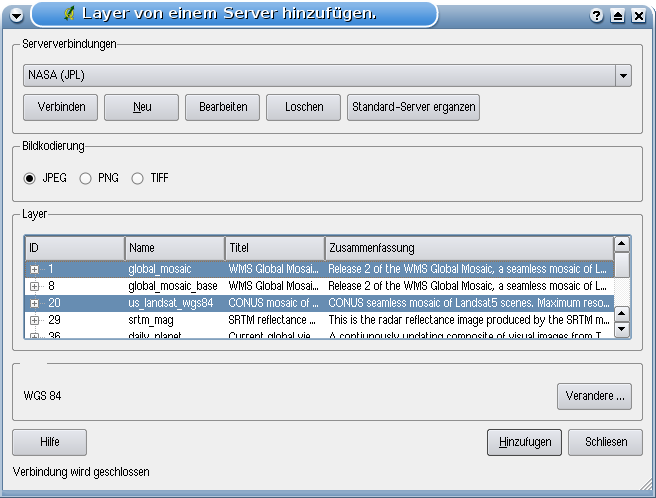
\includegraphics[clip=true,width=0.6\textwidth]{connection_wms}
  \caption{Dialog for adding a WMS server, showing its available layers \nixcaption}\label{fig:connection_wms}
\end{figure}

\minisec{Image Encoding}

The \tab{Image encoding} section now lists the formats that are supported by both
the client and server.  Choose one depending on your image accuracy requirements.

\begin{Tip}[ht]\caption{\textsc{Image Encoding}}
You will typically find that a WMS server offers you the choice
of JPEG or PNG image encoding.  JPEG is a lossy compression format,
whereas PNG faithfully reproduces the raw raster data.

Use JPEG if you expect the WMS data to be photographic in nature and/or you don't
mind some loss in picture quality.  This trade-off typically reduces by 5 times
the data transfer requirement compared to PNG.

Use PNG if you want precise representations of the original data, and you don't mind
the increased data transfer requirements.
\index{WMS!image encoding}
\end{Tip}

\minisec{Options}

The\tab{Options} section provides a text-field where you can add a name
for the WMS-layer. This name will be presented in the legend after loading
the layer.

If the OnlineRessource-URL from the GetCapabilities-document is different
from the given URL inside the connection-parameters, QGIS will ask you
which URL it should use. Depending on your answer QGIS will check the
checkboxes for yourself based on your answere. This can also be tweaked with a
\checkbox{Ignore GetMap URL} checkbox and a
\checkbox{Ignore GetFeatureInfo URL} checkbox separately, also later on.


\minisec{Layers} \label{ogc-wms-layers}

The \tab{Layers} tab lists the layers available from the selected
WMS server.  You may notice that some layers are expandible, this means
that the layer can be displayed in a choice of image styles.

You can select several layers at once, but only one image style per layer.
When several layers are selected, they will be combined at the WMS Server
and transmitted to QGIS in one go.

\begin{Tip}[ht]\caption{\textsc{WMS Layer Ordering}}
In this version of QGIS, WMS layers rendered by a server are overlaid
in the order listed in the Layers section, from top to bottom of the list.
If you want to change the overlay order, you can use the \tab{Layer Order} tab.
\index{WMS!remote server!layer ordering}
\end{Tip}

\minisec{Transparency}\label{ogc-wms-transparency}

In this version of QGIS, the transparency setting is hard-coded to
be always on, where available.

\begin{Tip}[ht]\caption{\textsc{WMS Layer Transparency}}
The availability of WMS image transparency depends on
the image encoding used:  PNG and GIF support transparency,
whilst JPEG leaves it unsupported.
\index{WMS!layer transparency}
\end{Tip}

\minisec{Coordinate Reference System}
\index{WMS!CRS}
\index{WMS!coordinate reference system}
\index{OGC!CRS}
\index{OGC!coordinate reference system}
\index{Projections!WMS}
\index{Projections!CRS}
\index{Projections!coordinate reference system}
\index{CRS}
\index{coordinate reference system}
\index{SRS}
\index{Projections!SRS}

A Coordinate Reference System (CRS) is the OGC terminology for a QGIS Projection.

Each WMS Layer can be presented in multiple CRSs, depending
on the capability of the WMS server.  You may notice that the \textsl{x} changes in
the \textsl{Coordinate Reference System (x available)} header as you
select and deselect layers from the \tab{Layers} section.

To choose a CRS, select \button{Change...} and a screen similar to
Figure \ref{fig:projections} in Section \ref{label_projstart} will appear.
The main difference with the WMS version of the screen is that only
those CRSs supported by the WMS Server will be shown.


\begin{Tip}[ht]\caption{\textsc{WMS Projections}}
For best results, make the WMS layer the first layer
you add to your project.  This allows the project
projection to inherit the CRS you used to render the WMS layer.
On-the-fly projection (see Section \ref{sec:projection-specifying})
can then be used to fit any subsequent
vector layers to the project projection.
In this version of QGIS, if you add a WMS layer later, and give it a different
CRS to the current project projection, unpredictable
results can occur.
\end{Tip}

%
% server-search tab.
%
\subsection{Server-Search}
\label{sec:serversearch}
\index{WMS!serversearch}
\index{WMS!search}
\index{OGC!search}

Within QGIS you can search for WMS-servers. Figure \ref{fig:searchtab} shows
the newly created \tab{search}-tab with the \dialog{Add Layer(s) from a
Server}-dialog.

\begin{figure}[ht]
  \centering
  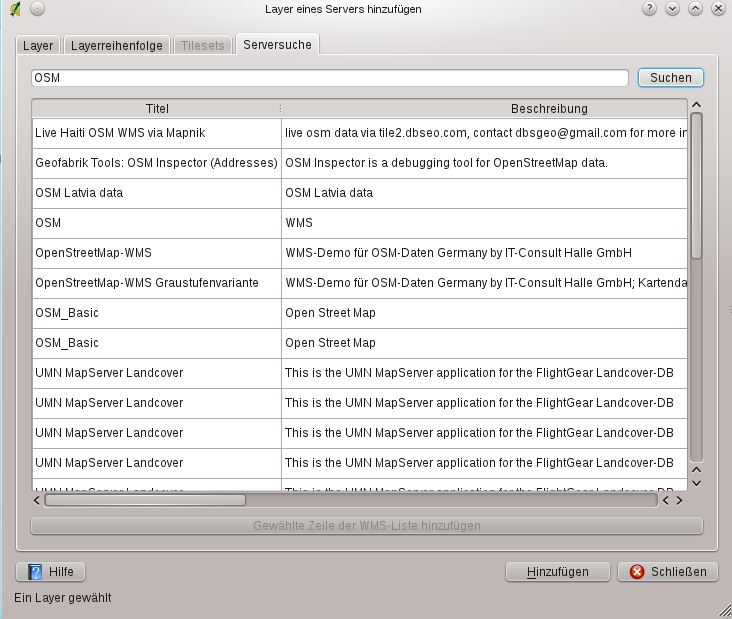
\includegraphics[clip=true,width=0.6\textwidth]{wms_server-search}
  	\caption{Dialog for searching WMS servers after some keywords \nixcaption}\label{fig:searchtab}
\end{figure}

As you can see it is possible to enter a search-string in the textfield an
hit the \button{Search} button.

After a short while the search result will be populated into the tab below
the textfield.

Browse the result list and inspect your searchresults within the table. To
visualize the results, select an table entry, press the \button{Add
selected row to WMS-list} button and change back to the \tab{server} tab.

QGIS automatically has updated your server list and the selected
searchresult is already enabled in the list of saved WMS-servers.

You only need to request the list of layers by clicking the
\button{Connect} button.

This option is quite handy when you want to search maps by specific
keywords.

Basically this option is a frontend to the API of
\url{http://geopole.org}.

%
% Layer Order
%
\subsection{Layer Order} \label{sec:layerorder}
\index{WMS!layerorder}

Within the tab \tab{Layer Order} you can select the drawing-order of the
selected layers. This comes handy when you have selected a list of layers from a
WMS-server and wanted to change the drawing-order of particular layers.

Just select the layer you want to change and press the up or down-button
above the layerlist.

%
% Tilesets
%
\subsection{Tilesets}\label{sec:tilesets}
\index{WMS!tileset}
\index{WMS!WMS-C}

When using WMS-C (Cached WMS) Services like
\url{http://labs.metacarta.com/wms-c/Basic.py} you are able to browse
through the \tab{tiles}-tab given by the server. Additional information like
tilesize, formats and supported CRS are listed in this table.

In combination with this feature you can use the tile scale slider from
the \mainmenuopt{View} \arrow \dropmenuopt{tile scale slider}, which gives you
the available scales from the tileserver with nice slider docked in.

%
% Identify
%
\subsection{Using the Identify Tool}\label{sec:ogc-wms-identify}
\index{WMS!identify}
\index{identify!WMS}
\index{WMS!GetFeatureInfo}

Once you have added a WMS server,
and if any layer from a WMS server is queryable, you can then use
the \toolbtntwo{mActionIdentify}{Identify} tool to select a pixel on the map canvas.
A query is made to the WMS server for each selection made.

The results of the query are returned in plain text.
The formatting of this text is dependent on the particular
WMS server used.

\subsubsection{Viewing Properties}\label{sec:ogc-wms-properties}\index{WMS!properties}
\index{rasters!properties}

Once you have added a WMS server, you can view its properties
by right-clicking on it in the legend, and selecting
\button{Properties}.


\minisec{Metadata Tab}\label{sec:ogc-wms-properties-metadata}
\index{rasters!metadata}
\index{WMS!metadata}
\index{WMS!capabilites}

The \tab{Metadata} tab displays a wealth of information about the WMS server,
generally collected from the Capabilities statement returned from
that server.

Many definitions can be gleaned by reading the WMS
standards \cite{OGCWMS010101web}, \cite{OGCWMS010300web}, but
here are a few handy definitions:

\begin{itemize}[label=--]
\item \textbf{Server Properties}

\begin{itemize}[label=--]
\item \textbf{WMS Version}      - The WMS version supported by the server.

\item \textbf{Image Formats}    - The list of MIME-types the server can respond with when
                                  drawing the map.  QGIS supports whatever formats
                                  the underlying Qt libraries were built with, which
                                  is typically at least \texttt{image/png}
                                  and \texttt{image/jpeg}.

\item \textbf{Identity Formats} - The list of MIME-types the server can respond with when
                                  you use the Identify tool.  Currently QGIS supports
                                  the \texttt{text-plain} type.

\end{itemize}

\item \textbf{Layer Properties}

\begin{itemize}[label=--]
\item \textbf{Selected}         - Whether or not this layer was selected when its                                                                        server was added to this project.

\item \textbf{Visible}          - Whether or not this layer is selected as visible
                                  in the legend.  (Not yet used in this version of QGIS.)

\item \textbf{Can Identify}     - Whether or not this layer will return any results
                                  when the Identify tool is used on it.

\item \textbf{Can be Transparent} - Whether or not this layer can be rendered with transparency.
                                    This version of
                                    QGIS will always use transparency if this is \textsl{Yes}
                                    and the image encoding supports transparency
% BM: doesn't seem to work?
%                                    (see Section
%                                    \ref{ogc-wms-transparency}
%                                    ).
                                    .

\item \textbf{Can Zoom In}      - Whether or not this layer can be zoomed in by the server.  This version
                                  of QGIS assumes all WMS layers have this set to \textsl{Yes}.
                                  Deficient layers may be rendered strangely.

\item \textbf{Cascade Count}    - WMS servers can act as a proxy to other WMS servers to get
                                  the raster data for a layer.  This entry shows how
                                  many times the request for this layer is forwarded to peer
                                  WMS servers for a result.

\item \textbf{Fixed Width}, \textbf{Fixed Height}
                                - Whether or not this layer has fixed source pixel dimensions.
                                  This version
                                  of QGIS assumes all WMS layers have this set to nothing.
                                  Deficient layers may be rendered strangely.

\item \textbf{WGS 84 Bounding Box} - The bounding box of the layer, in WGS 84 coordinates.
                                     Some WMS servers do not set this correctly (e.g. UTM
                                     coordinates are used instead).  If this is the case,
                                     then the initial view of this layer may be rendered
                                     with a very ``zoomed-out'' appearance by QGIS.
                                     The WMS webmaster should be informed of this error,
                                     which they may know as the WMS XML elements
                                     \texttt{LatLonBoundingBox},
                                     \texttt{EX\_GeographicBoundingBox} or
                                     the CRS:84 \texttt{BoundingBox}.

\item \textbf{Available in CRS} - The projections that this layer can be rendered in by
                                  the WMS server.  These are listed in the WMS-native format.

\item \textbf{Available in style} - The image styles that this layer can be rendered in by
                                    the WMS server.

\end{itemize}

\end{itemize}


\subsection{WMS Client Limitations}\label{sec:ogc-wms-limits}\index{WMS!client!limits}

Not all possible WMS Client functionality had been included in this version of QGIS.
Some of the more notable exceptions follow:

\minisec{Editing WMS Layer Settings}
\index{WMS!layer settings!editing}

Once you've completed the \toolbtntwo{mActionAddWmsLayer}{Add WMS layer}
procedure, there is no ability to change the settings.

A workaround is to delete the layer completely and start again.

\minisec{WMS Servers Requiring Authentication}
\index{WMS!remote server!authentication}
\index{WMS!remote server!basic authentification}

Currently public accessible and secured WMS-services are supported.
The secured WMS-servers can be accessed by public authentification. You
can add the (optional) credentials when you add a WMS-server. See section
\ref{sec:ogc-wms-servers} for details.

\begin{Tip}[ht]\caption{\textsc{Accessing secured OGC-layers}}
If you need to access secured layers with other secured methods
than basic authentification, you could use InteProxy as
a transparent proxy, which does supports several authentification methods.
More information can be found at the InteProxy-manual found on the website
\url{http://inteproxy.wald.intevation.org}.
\index{WMS!secured layers!}\index{OGC!Authentication}
\end{Tip}


%
% WMS-server
%

\section{WMS Server}\label{sec:ogc-wmsserver}
\index{WMS!server}

QGIS mapserver is an open source WMS 1.3 implementation which, in addition,
implements advanced cartographic features for thematic mapping. The QGIS
mapserver is a FastCGI/CGI (Common Gateway Interface) application written in
C++ that works together with a webserver (e.g. Apache, Lighttpd). 


It uses QGIS as backend for the GIS logic and for map rendering. Furthermore the 
Qt library is used for graphics and for platform independent 
C++ programming. In contrast to other WMS software, the QGIS mapserver uses 
cartographic rules in SLD/SE as a configuration language, both for the server 
configuration and for the user-defined cartographic rules. 

Moreover, the QGIS mapserver project provides the “Publish to Web” plugin, a 
plugin for QGIS desktop which exports the current layers and symbology as a 
web project for QGIS mapserver (containing cartographic visualisation rules 
expressed in SLD).

As QGIS desktop and QGIS mapserver use the same visualization libraries, the
maps that are published on the web look the same as in desktop GIS. The 
Publish to Web plugin currently supports basic symbolization, with more complex 
cartographic visualisation rules introduced manually. As the configuration is 
performed with the SLD standard and its documented extensions, there is only 
one standardised language to learn, which greatly simplifies the complexity 
of creating maps for the Web.

Further information is available at: \\
\url{http://karlinapp.ethz.ch/qgis\_wms/} \\
\url{http://www.qgis.org/wiki/QGIS\_mapserver\_tutorial} \\
\url{http://linfiniti.com/2010/08/qgis-mapserver-a-wms-server-for-the-masses/}



%
% WFS-client
%
\section{WFS and WFS-T Client}\label{sec:ogc-wfs}
\index{WFS!WFS-T}
\index{WFS!Transactional}

In QGIS, a WFS layer behaves pretty much like any other vector layer. You
can identify and select features and view the attribute table. Since QGIS 1.6 
editing (WFS-T) is also supported, if the server provides this feature. To start 
the WFS plugin you need to open \mainmenuopt{Plugins} \arrow 
\dropmenuopttwo{mActionShowPluginManager}{Plugin Manager...}, activate the 
\checkbox{WFS plugin} checkbox and click \button{OK}.

A new \toolbtntwo{mIconAddWfsLayer}{Add WFS Layer} icon appears next
to the WMS icon. Click on it to open the dialog. In general adding a WFS
layer is very similar to the procedure used with WMS. The difference is
there are no default servers defined, so we have to add our own.

\subsubsection{Loading a WFS Layer}

As an example we use the DM Solutions WFS server and display a layer. The URL is:
\begin{verbatim}
http://www2.dmsolutions.ca/cgi-bin/mswfs_gmap
\end{verbatim}

\begin{enumerate}
  \item Make sure the WFS plugin is loaded; if not, open the Plugin Manager and load it
  \item Click on the
  \toolbtntwo{mIconAddWfsLayer}{Add WFS Layer}
  tool on the plugins toolbar
  \item Click on \button{New}
  \item Enter \inputtext{Name}{DM Solutions} as the name
  \item Enter the URL (see previous page)
  \item Click \button{OK}
  \item Choose \selectstring{Server Connections}{DM Solutions} from the drop-down box
  \item Click \button{Connect}
  \item Wait for the list of layers to be populated
  \item Click on the \clicklistitem{Parks} layer
  \item Click \button{Ok} to add the layer to the map
  \item Wait patiently for the features to appear
\end{enumerate}

Note that the WFS-plugin also recognizes the proxy-settings you have set
in your preferences.

\begin{figure}[ht]
  \centering
  	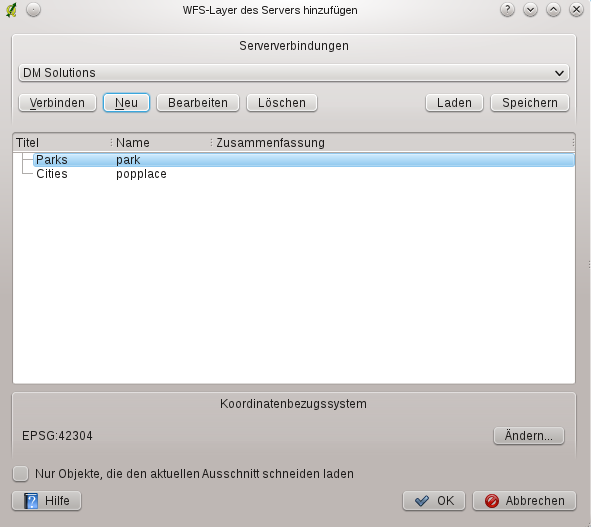
\includegraphics[clip=true,width=0.45\textwidth]{connection_wfs}
  	\caption{Adding a WFS layer \nixcaption}\label{fig:wfs_dmsolutions}
\end{figure}

Without using the checkbox \checkbox{Only request features overlapping the
current view extent} QGIS fetches all features from the WFS-server. If you
only want to have a small selection based on your extent, zoom to the area
of interest, request the WFS-layer again and make sure you have checked
the checkbox mentioned above. Basically this addes the BBOX-parameter with
the values from you current extent to the WFS-query. This is extremly
usefull when you only want to request \textbf{some} features from a huge
WFS-dataset.

You'll notice the download progress is visualized in the left bottom of the 
QGIS main window. Once the layer is loaded, you can identify and select a 
province or two and view the attribute table.

Remember this plugin works best with MapServer WFS servers. It still
could be, that you might experience random behavior
and crashes. You can look forward to improvements in a future version of the plugin.

This means that only WFS 1.0.0 is supported. At this point there have not
been many test against WFS versions implemented in other WFS-servers.
If you encounter problems with any other WFS-server, please do not
hesitate to contacting the development team. Please refer to Section
\ref{label_helpsupport} for further information about the mailinglists.

\begin{Tip}[htb]\caption{\textsc{Finding WFS Servers}}
You can find additional WFS servers by using Google or your
favorite search engine. There are a number of lists with public URLs, some
of them maintained and some not.
\index{WFS!remote server!}
\end{Tip}

\begin{Tip}[htb]\caption{\textsc{Accessing secure WFS Servers}}
Within the dialog \dialog{Create a new WFS-connection} QGIS does not support
authenficated WFS-connections yet. Within one of the next releases we expect
to also support authenticated WFS-servers. Meanwhile you could use InteProxy
(\url{http://inteproxy.wald.intevation.org}) for accessing authenticated
WFS-servers.
\index{WFS!authenticate remote server!}
\index{WFS!secured WFS server!}
\end{Tip}

\FloatBarrier
